\documentclass[tikz,border=4pt]{standalone}

\usepackage{amsmath}
\usepackage{amssymb}
\usepackage{xcolor}
\usepackage{tikz}


\usetikzlibrary{
    arrows,
    arrows.meta,
    automata,
    backgrounds,
    calc,
    decorations.pathreplacing,
    fit,
    matrix,
    positioning,
    shapes,
    shapes.arrows,
    shapes.geometric,
    shapes.multipart
}



\tikzset{
  start/.style={
    rectangle,
    rounded corners,
    minimum width=3.5cm,
    minimum height=1cm,
    text centered,
    text width=3cm,
    draw=black,
    fill=green!20
  },
  stop/.style={
    rectangle,
    rounded corners,
    minimum width=3cm,
    minimum height=1cm,
    text centered,
    text width=2.5cm,
    draw=black,
    fill=red!20
  },
  decision/.style={
    diamond,
    aspect=2,
    minimum width=3cm,
    minimum height=1.2cm,
    text centered,
    text width=2.5cm,
    inner sep=1pt,
    draw=black,
    fill=yellow!20
  },
  process/.style={
    rectangle,
    minimum width=3cm,
    minimum height=1cm,
    text centered,
    text width=2.7cm,
    draw=black,
    fill=blue!10
  },
  arrow/.style={
    thick,
    -{Stealth}
  }
}


\usetikzlibrary{
  arrows.meta,
  positioning,
  shapes.geometric
}

\tikzset{
  start/.style={
    rectangle,
    rounded corners,
    minimum width=3.5cm,
    minimum height=1cm,
    text centered,
    text width=3cm,
    draw=black,
    fill=green!20
  },
  stop/.style={
    rectangle,
    rounded corners,
    minimum width=3cm,
    minimum height=1cm,
    text centered,
    text width=2.5cm,
    draw=black,
    fill=red!20
  },
  decision/.style={
    diamond,
    aspect=2,
    minimum width=3cm,
    minimum height=1.2cm,
    text centered,
    text width=2.5cm,
    inner sep=1pt,
    draw=black,
    fill=yellow!20
  },
  io/.style={
    trapezium,
    trapezium left angle=70,
    trapezium right angle=110,
    minimum width=3.5cm,
    minimum height=1cm,
    text centered,
    text width=3cm,
    draw=black,
    fill=blue!20
  },
  arrow/.style={
    thick,
    -{Stealth}
  }
}


\begin{document}

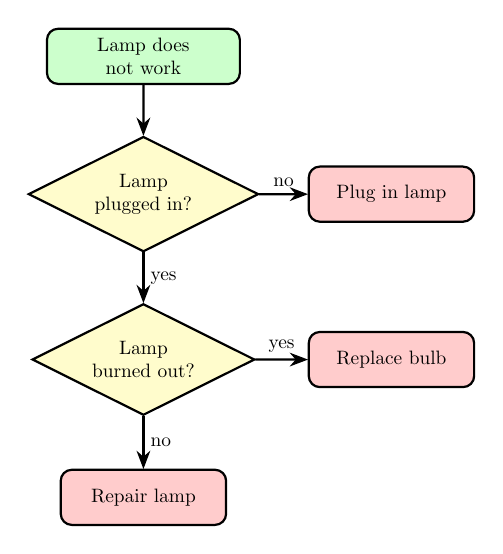
\begin{tikzpicture}[node distance=2.5cm, thick,scale=1.4, every node/.style={scale=0.7}]
    \node (start) [start] {Lamp does not work};
    \node (plugged) [decision, below of=start] {Lamp plugged in?};
        \node (plug) [stop, right of=plugged, xshift=2cm] {Plug in lamp};
    \node (burned) [decision, below of=plugged, yshift=-0.5cm] {Lamp burned out?}; 
        \node (replace) [stop, right of=burned, xshift=2cm] {Replace bulb}; 
    \node (repair) [stop, below of=burned] {Repair lamp};

    \draw [arrow] (start) -- (plugged);
    \draw [arrow] (plugged) -- node[anchor=west] {yes} (burned);
    \draw [arrow] (plugged) -- node[anchor=south] {no} (plug);
    \draw [arrow] (burned) -- node[anchor=south] {yes} (replace);
    \draw [arrow] (burned) -- node[anchor=west] {no} (repair);
  \end{tikzpicture}

\end{document}
